\chapter{The CMS Detector}
\label{chap:detector}

The interactions of the protons more often than not are just glancing blows off one another, there is not much energy transfer and the protons generally remain intact. The CMS experiment is predominantly interested in the dynamics of collisions with a very large energy transfer, unveiling quarks and gluons that are within the proton. Large energy transfers are necessary for the creation of massive particles such as the electroweak bosons, or potentially a new particle not within the SM. These high-energy collisions result in particles with a large amount of momentum in the direction perpendicular to the beam line ($p_{T}$), where the components of the CMS detector are carefully arranged. By detecting the outgoing flux of particles from these high-energy events, we are able to reconstruct the dynamics and quantum mechanical processes involved in the proton interactions.

The detector is composed of a modular design of subsystems allowing for measurements of a wide spectra of particles. As seen in Figure \ref{fig:howcmsworks}, these detectors are placed around the interaction point to collect as much of the collision remnants as possible. In this figure, the beam line is seen as a small grey tube extending from the bottom right towards the top left. The interaction point is within the silicon trackers.

Each different system is capable of detecting specific types of particles. A silicon tracker allows for the reconstruction of charged particles traveling at least $50\,\mathrm{cm}$ (e.g. electrons $e^{\pm}$, charged pions $\pi^{\pm}$); calorimeters measure the energy of hadrons (e.g. protons, $K^{0}_{L}$) and photons $\gamma$; muon $\mu^{\pm}$ identification is made with gas detectors. The particle identification exploits the unique signature each of these particles leave in our detector. Figure~\ref{fig:schematicview} illustrates these signatures for some common SM particles. 

Many of the particles produced in the interaction are unstable and decay before traveling any appreciable distance in the detector. These particles, such as top quarks, electroweak bosons, and many hadrons, must be reconstructed by the identification of their decay products. For instance, a Z boson may be reconstructed as a pair of oppositely charged muons $\mu^{\pm}$.

This chapter will discuss the main elements of the CMS detector, beginning with the innermost (closest to the beam pipe) silicon tracker and concluding with the muon system. The detector can generically be divided into central \textit{barrel} and forward \textit{endcap} regions. The geometry either takes the form of concentric cylinders (in the barrel) or flat planes of detectors (in the endcaps). This is most apparent in Figure~\ref{fig:detectoreta}, where the beamline is seen as the thin cyan line at the bottom of the image. The origin is defined as the center of the detector. The radial coordinate $r$ is the distance from the beam line, in the transverse plane. The z axis is the direction parallel to the beamline, counterclockwise when viewed from above. The coordinate $\eta\equiv-\tan{\ln{\theta/2}}$ is used to represent the polar angle above the beamline. The $\phi$ coordinate is the azimuth angle about the beamline, with $\phi=0$ aligning with the x-axis pointing towards the center of the LHC ring. The y-axis points up.

\begin{figure}
\centering
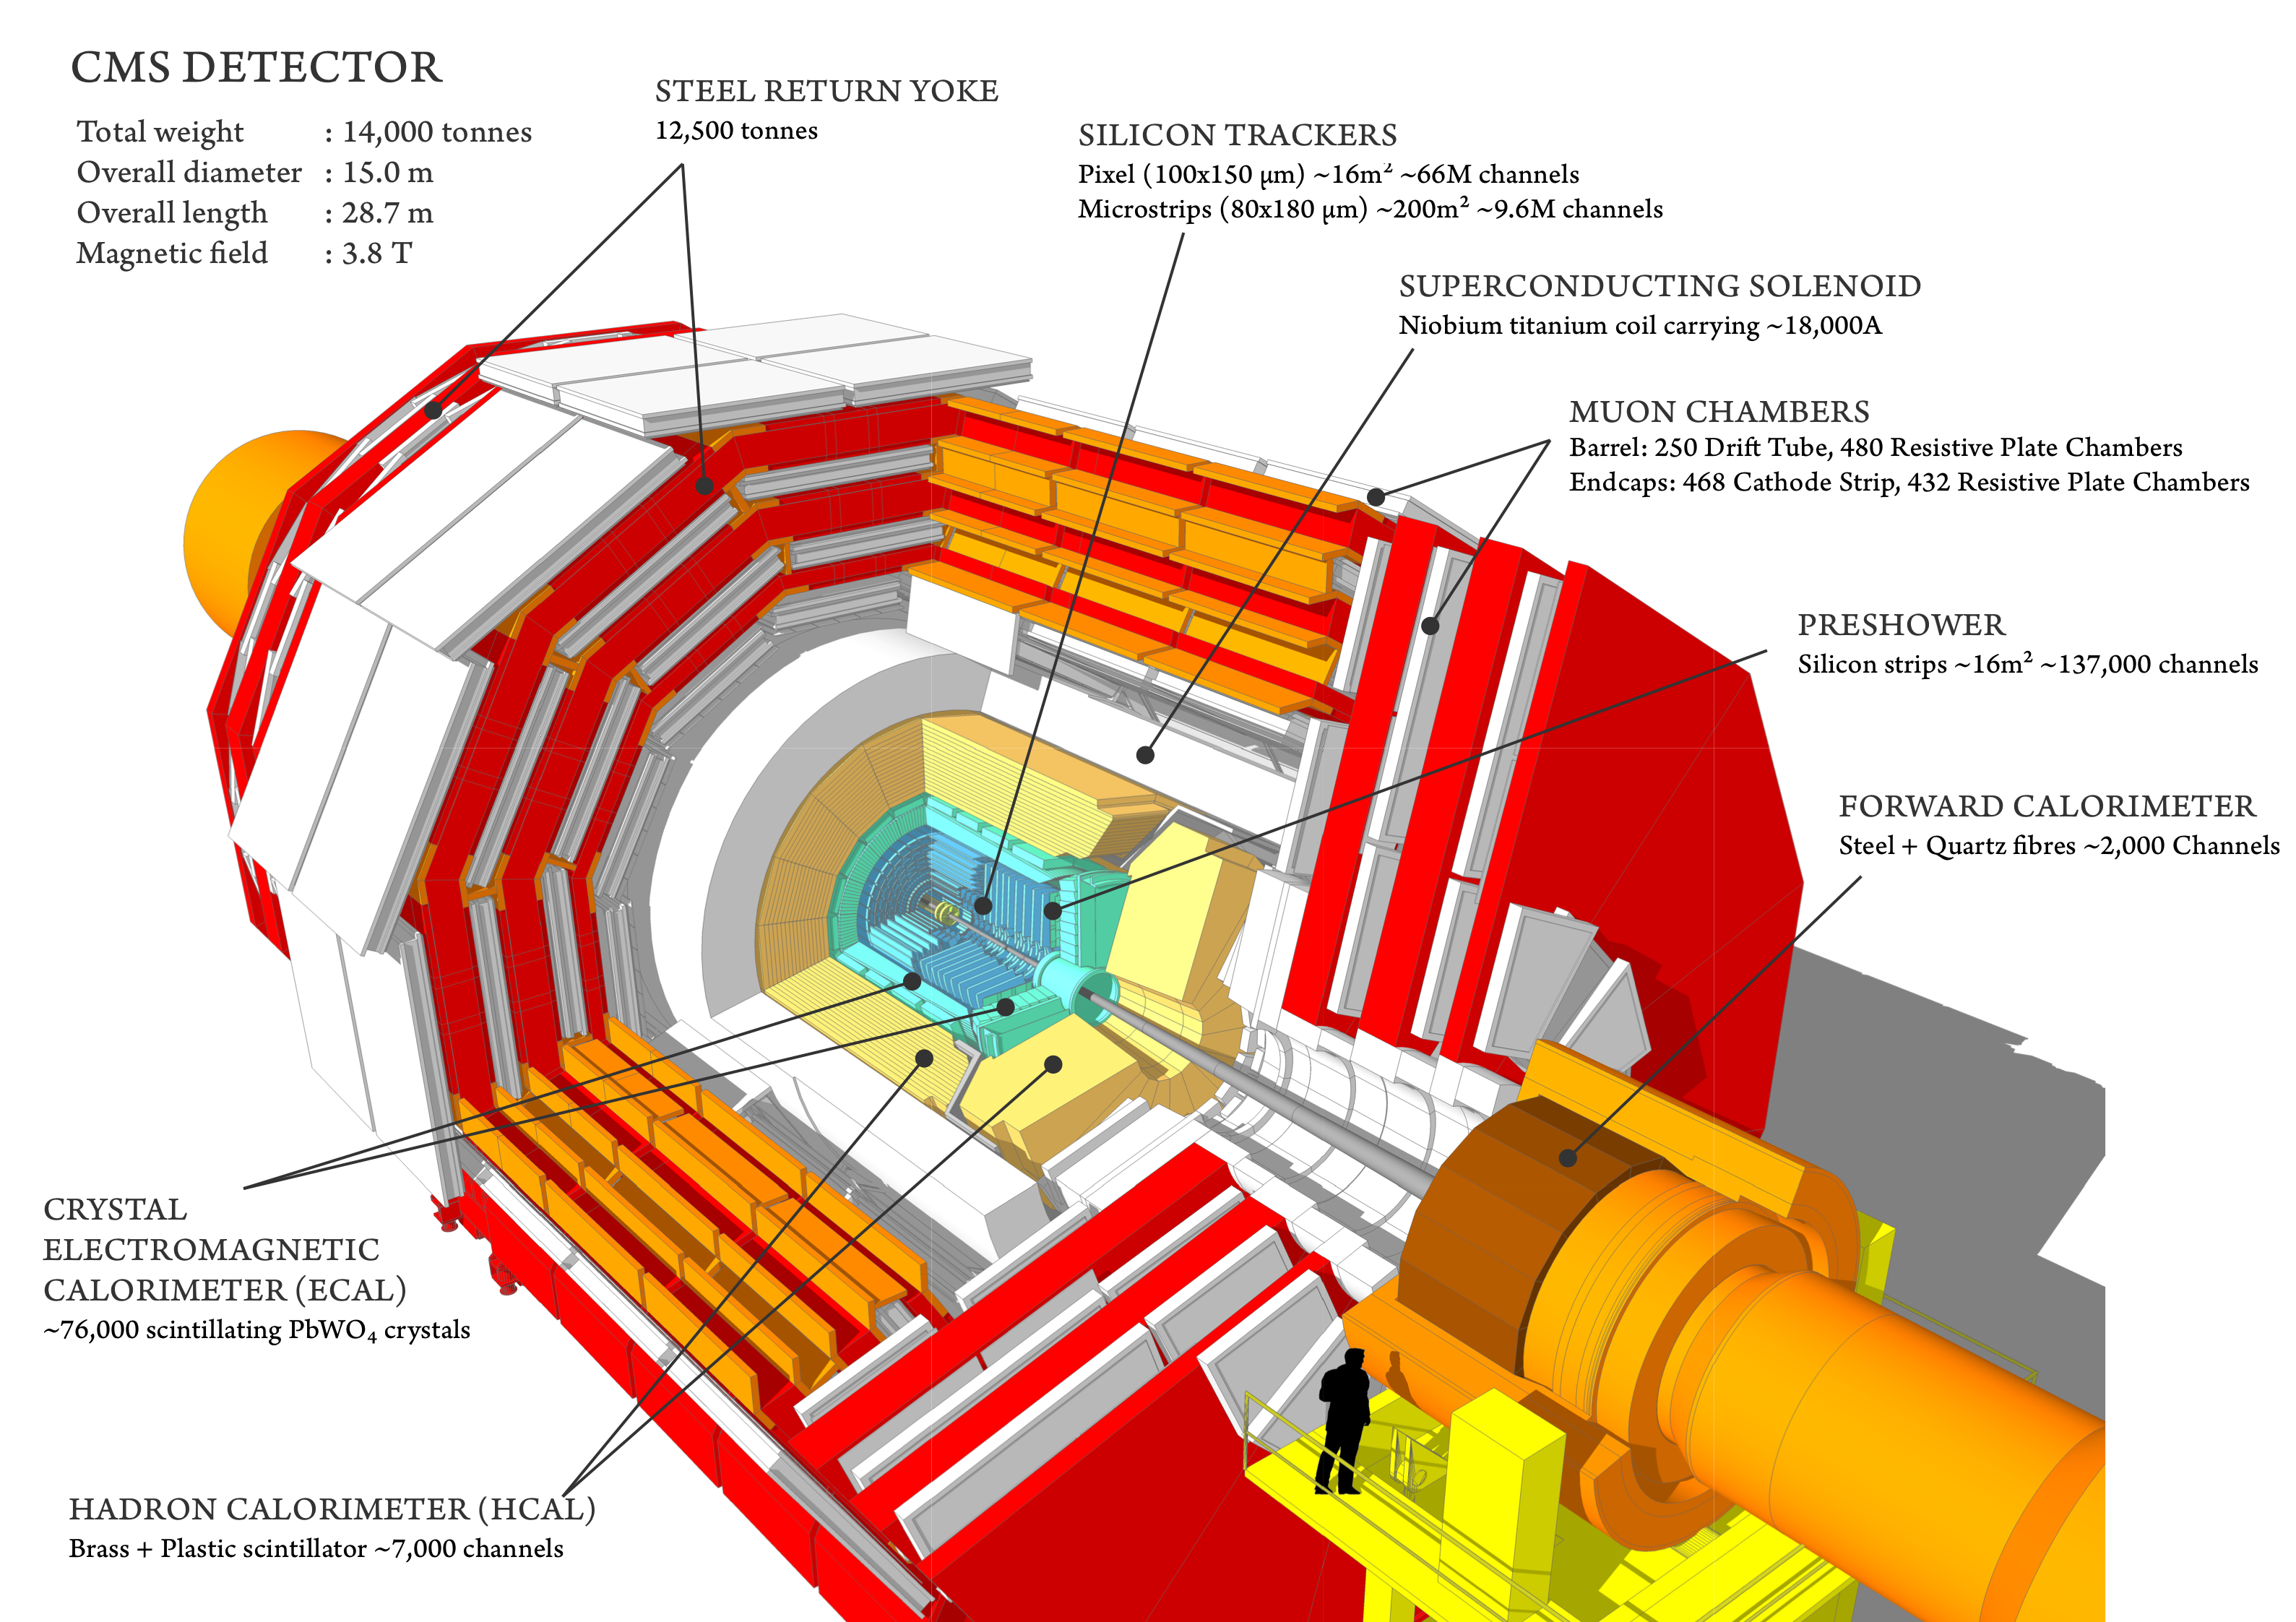
\includegraphics[width=0.75\textwidth]{figs/howcmsworks.png}
\caption[A diagram of the CMS detector.]{A diagram of the CMS detector. Specific detector subsystems are labeled.}
\label{fig:howcmsworks}
\end{figure}

\begin{figure}
\centering
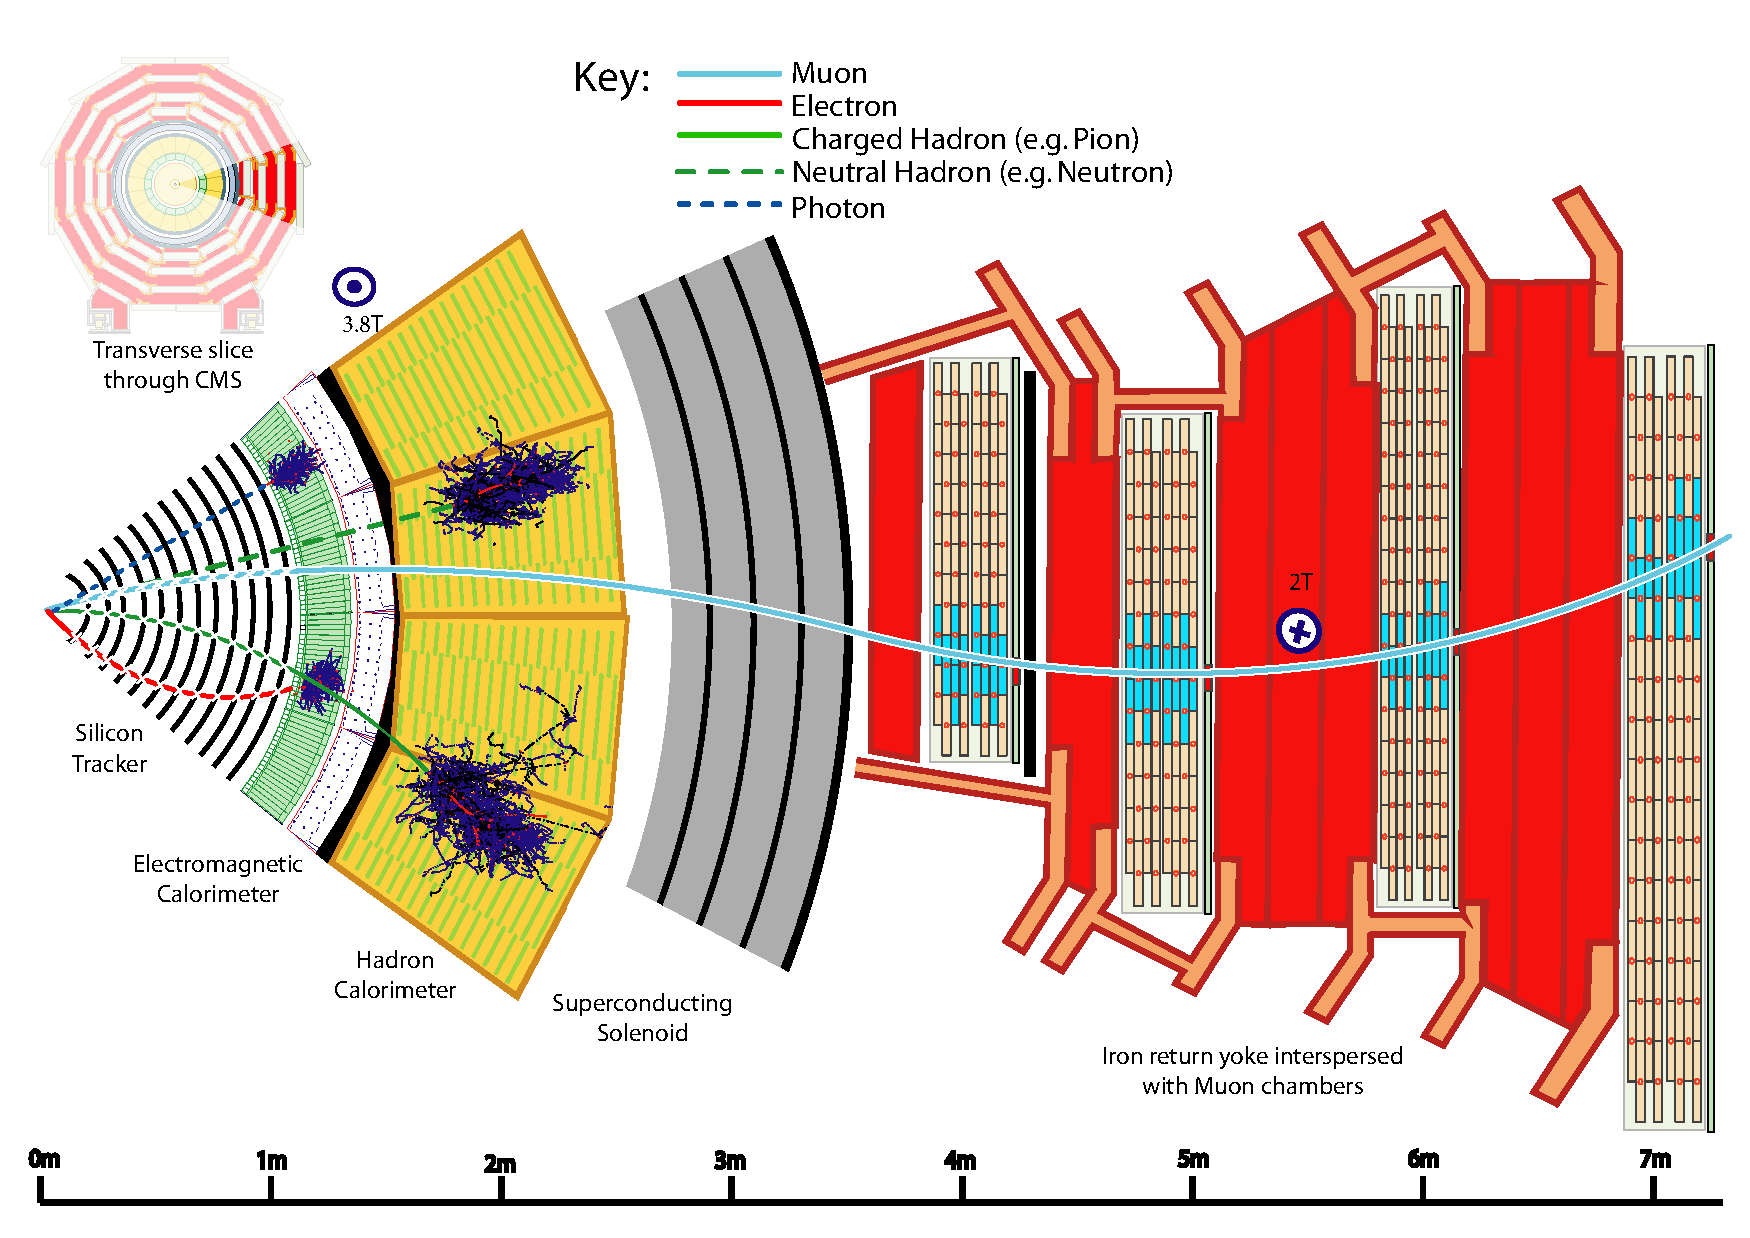
\includegraphics[width=0.75\textwidth]{figs/CMS-PRF-14-001_Figure_001.pdf}
\caption[A diagram of the CMS detector in the r-$\phi$ plane; particle signatures are shown.]{A diagram of the CMS detector in the r-$\phi$ plane; the beam axis is perpendicular to the page; SM particle signatures within the detector are shown.}
\label{fig:schematicview}
\end{figure}

\begin{figure}
\centering
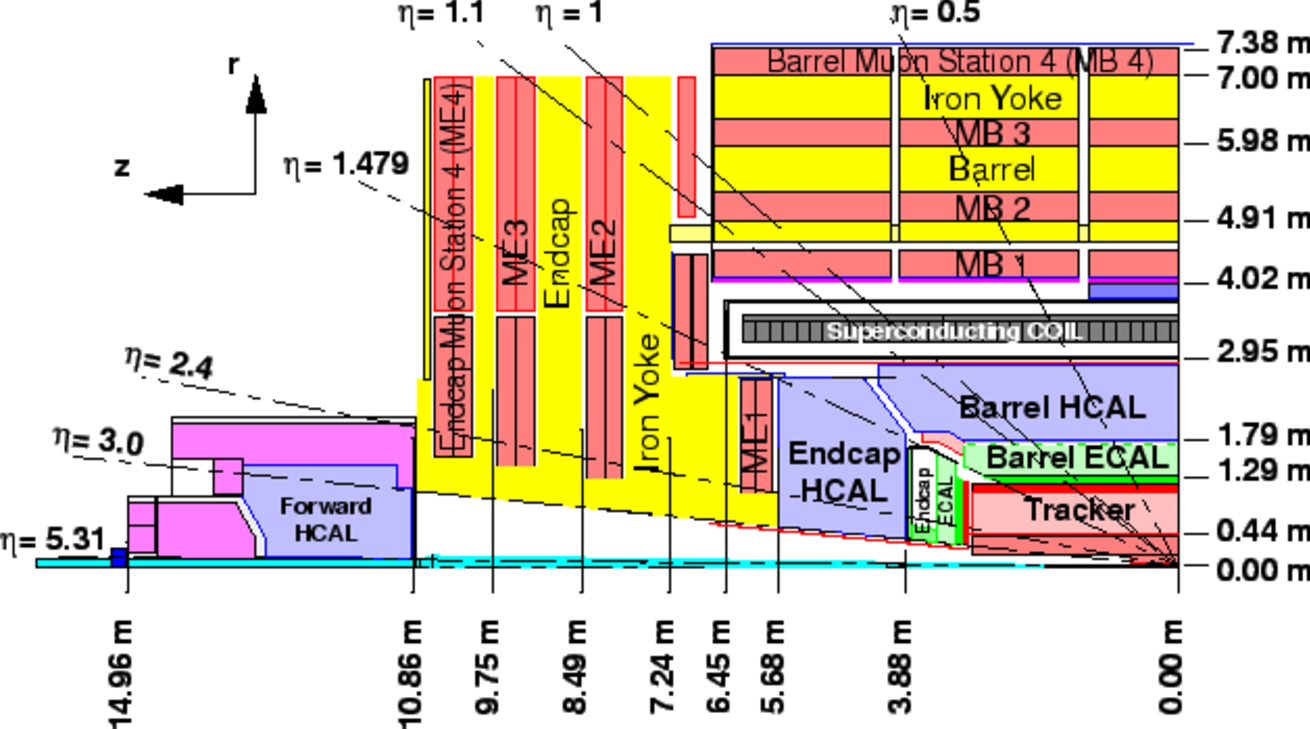
\includegraphics[width=0.75\textwidth]{figs/img41.pdf}
\caption[A diagram of the CMS detector in the r-z plane.]{A diagram of the CMS detector in the r-z plane; the beampipe is the thin cyan sliver along the bottom. The detector subtends a large solid angle about the interaction region.}
\label{fig:detectoreta}
\end{figure}

\section{Silicon Tracker}

The silicon tracker is responsible for the reconstruction of charged particles, which are mainly electrons, muons, kaons and pions. The particle trajectory is reconstructed using ionization deposits left in layers of thin silicon. The particle momentum is measured by the curvature of the trajectory when immersed in the magnetic field. The silicon tracker is divided into two major components. The pixel detector is at a closer proximity to the beam line and has finer spatial segmentation. The strips detector covers a much larger spatial volume and is responsible for the majority of the hits along a particle trajectory. \cite{trackertdr, trackertdradd}. A diagram of the geometry and layers of the tracker is seen in Figure~\ref{fig:tracker}.

The tracker is built of modules consisting of a layer of sensitive silicon bonded on top readout electronics. The silicon is arranged as a p-n junction, reversed-biased and fully-depleted. As a charged particle travels through the material, it ionizes the silicon creating electron-hole pairs within the depletion zone. Electric fields accelerate the charge through the silicon to the readout electronics bonded to the back of the sensor. The readout chips amplify, digitize, and store the hit information before being piped outside the detector. The silicon is very thin ($\sim300\,\mu m$), the tracker is constructed of as little material as possible so as not to perturb the trajectory of the particle.

\begin{figure}
\centering
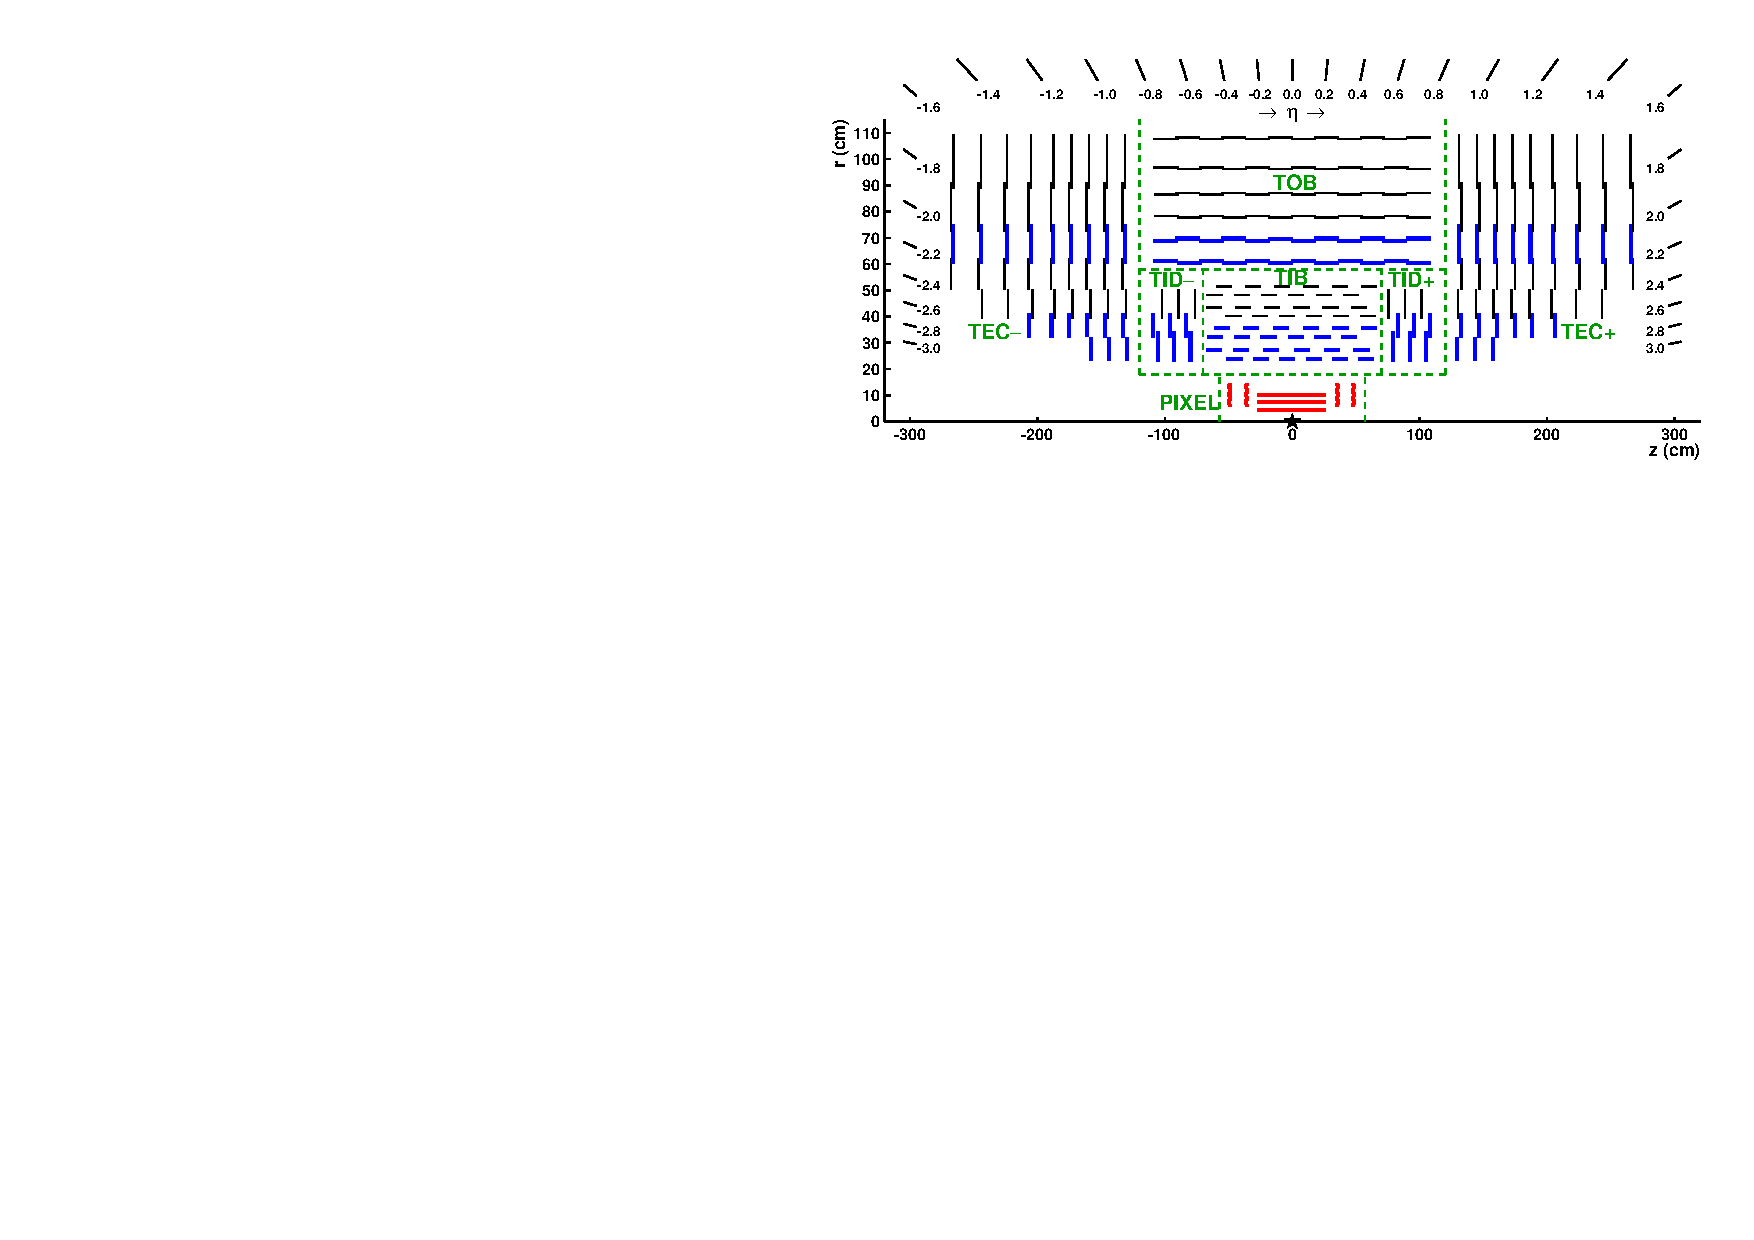
\includegraphics[width=0.8\textwidth]{figs/TrackerLayoutNew.pdf}
\caption[The CMS silicon tracker]{The CMS silicon tracker. The vertical and horizontal lines represent layers of silicon modules. Lines in blue represent layers with ``stereo'' hits, formed from two silicon layers.}
\label{fig:tracker}
\end{figure}

\subsection{Pixel Detector}

The task of the pixel detector is to provide the spatial granularity required for precision track vertexing. The barrel region ($|\eta|<1.5$) of the pixel detector consists of 3 concentric cylinders sitting at radii of 4.4, 7.3, and 10.2 cm from the beamline. The endcaps ($1.5<|\eta|<2.5$) consist of two discs on each side ($\pm$z) placed at $z = \pm 35.5, 48.5\,\textrm{cm}$. A pixel module, used to form the detector layers, consists of 16 readout chips glued to a $2\times6\,cm$ mechanical support structure. Bump-bonded to the readout chips are the $285\,\mu m$ thick silicon sensors. The readout chips and sensor are divided up into $100x150\mu\,m$ pixels which allow the excellent hit resolution (over 65 million channels for the entire detector). The $100\mu\,m$ lengths are oriented to give the most precise measurement of the $\phi$ coordinate of the track, as that is the direction on bending due to the magnetic field.  

A new pixel detector was installed in 2016 to accommodate the ever-increasing instantaneous luminosity provided by the LHC \cite{newpixel}. The increase in the luminosity results in many more additional proton-proton interactions per bunch crossing, called \textit{pileup}.  High pileup results in a very dense environment for track reconstruction to operate as all the individual hits in the detector layers must be disentangled correctly. To increase the performance, the new detector therefore included \textbf{4} layers in the barrel and \textbf{3} endcap discs on either end. The readout chip was upgraded to fully digital readout to give larger hit buffers to accommodate the increased hit rate.

\subsection{Strips Detector}

The silicon strips detector sits immediately outside the pixel detector and provides additional hits along a particle's trajectory. The barrel region ($|\eta|<1.5$) provides 10 layers of sensor situated between 20 and 116cm from the beamline. The endcap regions ($1.5<|\eta|<2.5$) have a total of 12 layers situated between 58 and 282cm from the center of the detector, on each side. The silicon modules are partitioned in roughly 10cm long strips which are oriented parallel to the beamline. The strip pitch varies ranging from $80-180\,\mu$m wide. The silicon thickness ranges from 320 to 500 $\mu\,m$ thick. Some of the layers, indicated in the blue lines in Figure \ref{fig:tracker}, have two modules which are slightly rotated relative to each other to give a ``stereo-hit'', providing a more precise position measurement.

\section{Electromagnetic Calorimeter}

The electromagnetic calorimeter is responsible for the reconstruction of electrons $e^{\pm}$ and photons $\gamma$. The energy is measured by collecting the light generated by an electromagnetic shower as the particle is absorbed in the calorimeter \cite{ecaltdr, ecaltdradd}. 

Electromagnetic showers are created when high energy photons or electrons enter the material comprising the ECAL. The cross section for interactions of these particles with the detector scales with the square of the atomic nucleus, it was for this reason that the material is made of clear PbWO$_{4}$ crystals. High energy photons in the detector predominantly lose energy by the creation of $e^{+}e^{-}$ pairs via interactions with detector bulk. The predominant energy loss for high-energy electrons is through the emission of \textit{bremsstrahlung}, or electromagnetic radiation created by the scattering of the electrons. An incident particle will therefore cause a shower in the detector as the interactions proceed until all the particles are sufficiently low energy and absorbed by the photodetectors mounted at the end of each crystal. Avalanche photodiodes with a gain of 50 and vacuum phototriodes with a gain of 10 are used in the barrel and endcap, respectively. The signal is then further amplified and digitized.

The electromagnetic calorimeter is divided into barrel ($|\eta|<1.5$) and endcap ($1.5<|\eta|<3$) regions comprising 75,848 crystals. The crystals measure 2.2$\,$x$\,$2.2$\,$x$\,$23$\,$cm in the barrel and 3$\,$x$\,$3$\,$x$\,$22$\,$cm in the endcaps; they are oriented radially outward from the interaction region. A schematic of the detector is seen in Figure~\ref{fig:ecal}. Additionally, the electromagnetic calorimeter serves as an absorber for the hadronic calorimeter, initiating a shower in approximately 1/3 of the hadrons that are headed the HCAL.

\begin{figure}
\centering
\begin{subfigure}[c]{0.35\textwidth}
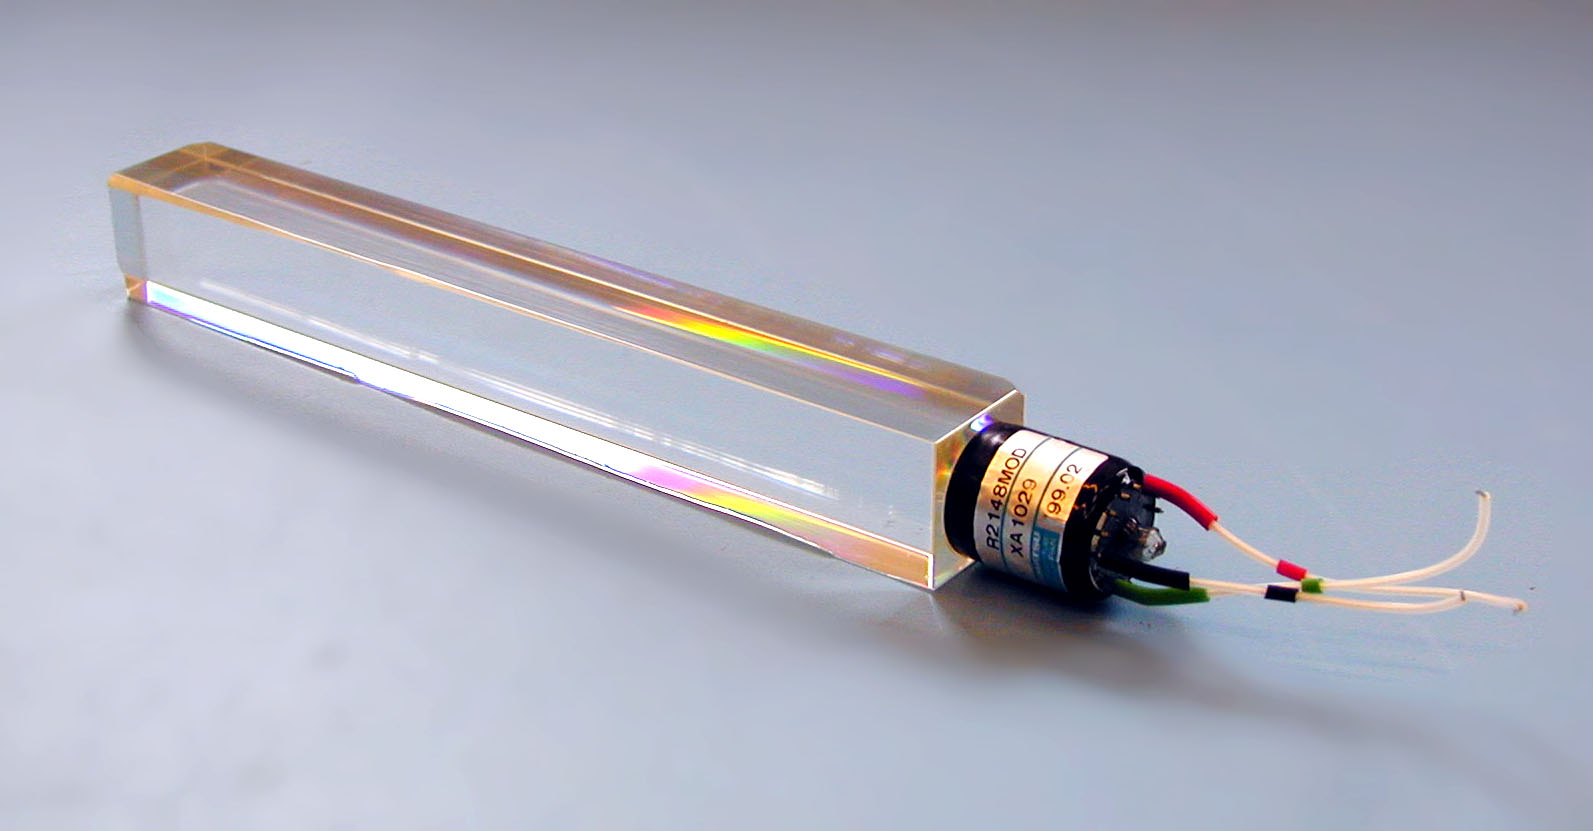
\includegraphics[width=\textwidth]{figs/ecalcrystal.jpg}
\caption{A single PbWO$_{4}$ crystal attached to photomultiplier tube.}
\label{fig:ecalcrystal}
\end{subfigure}
\begin{subfigure}[c]{0.625\textwidth}
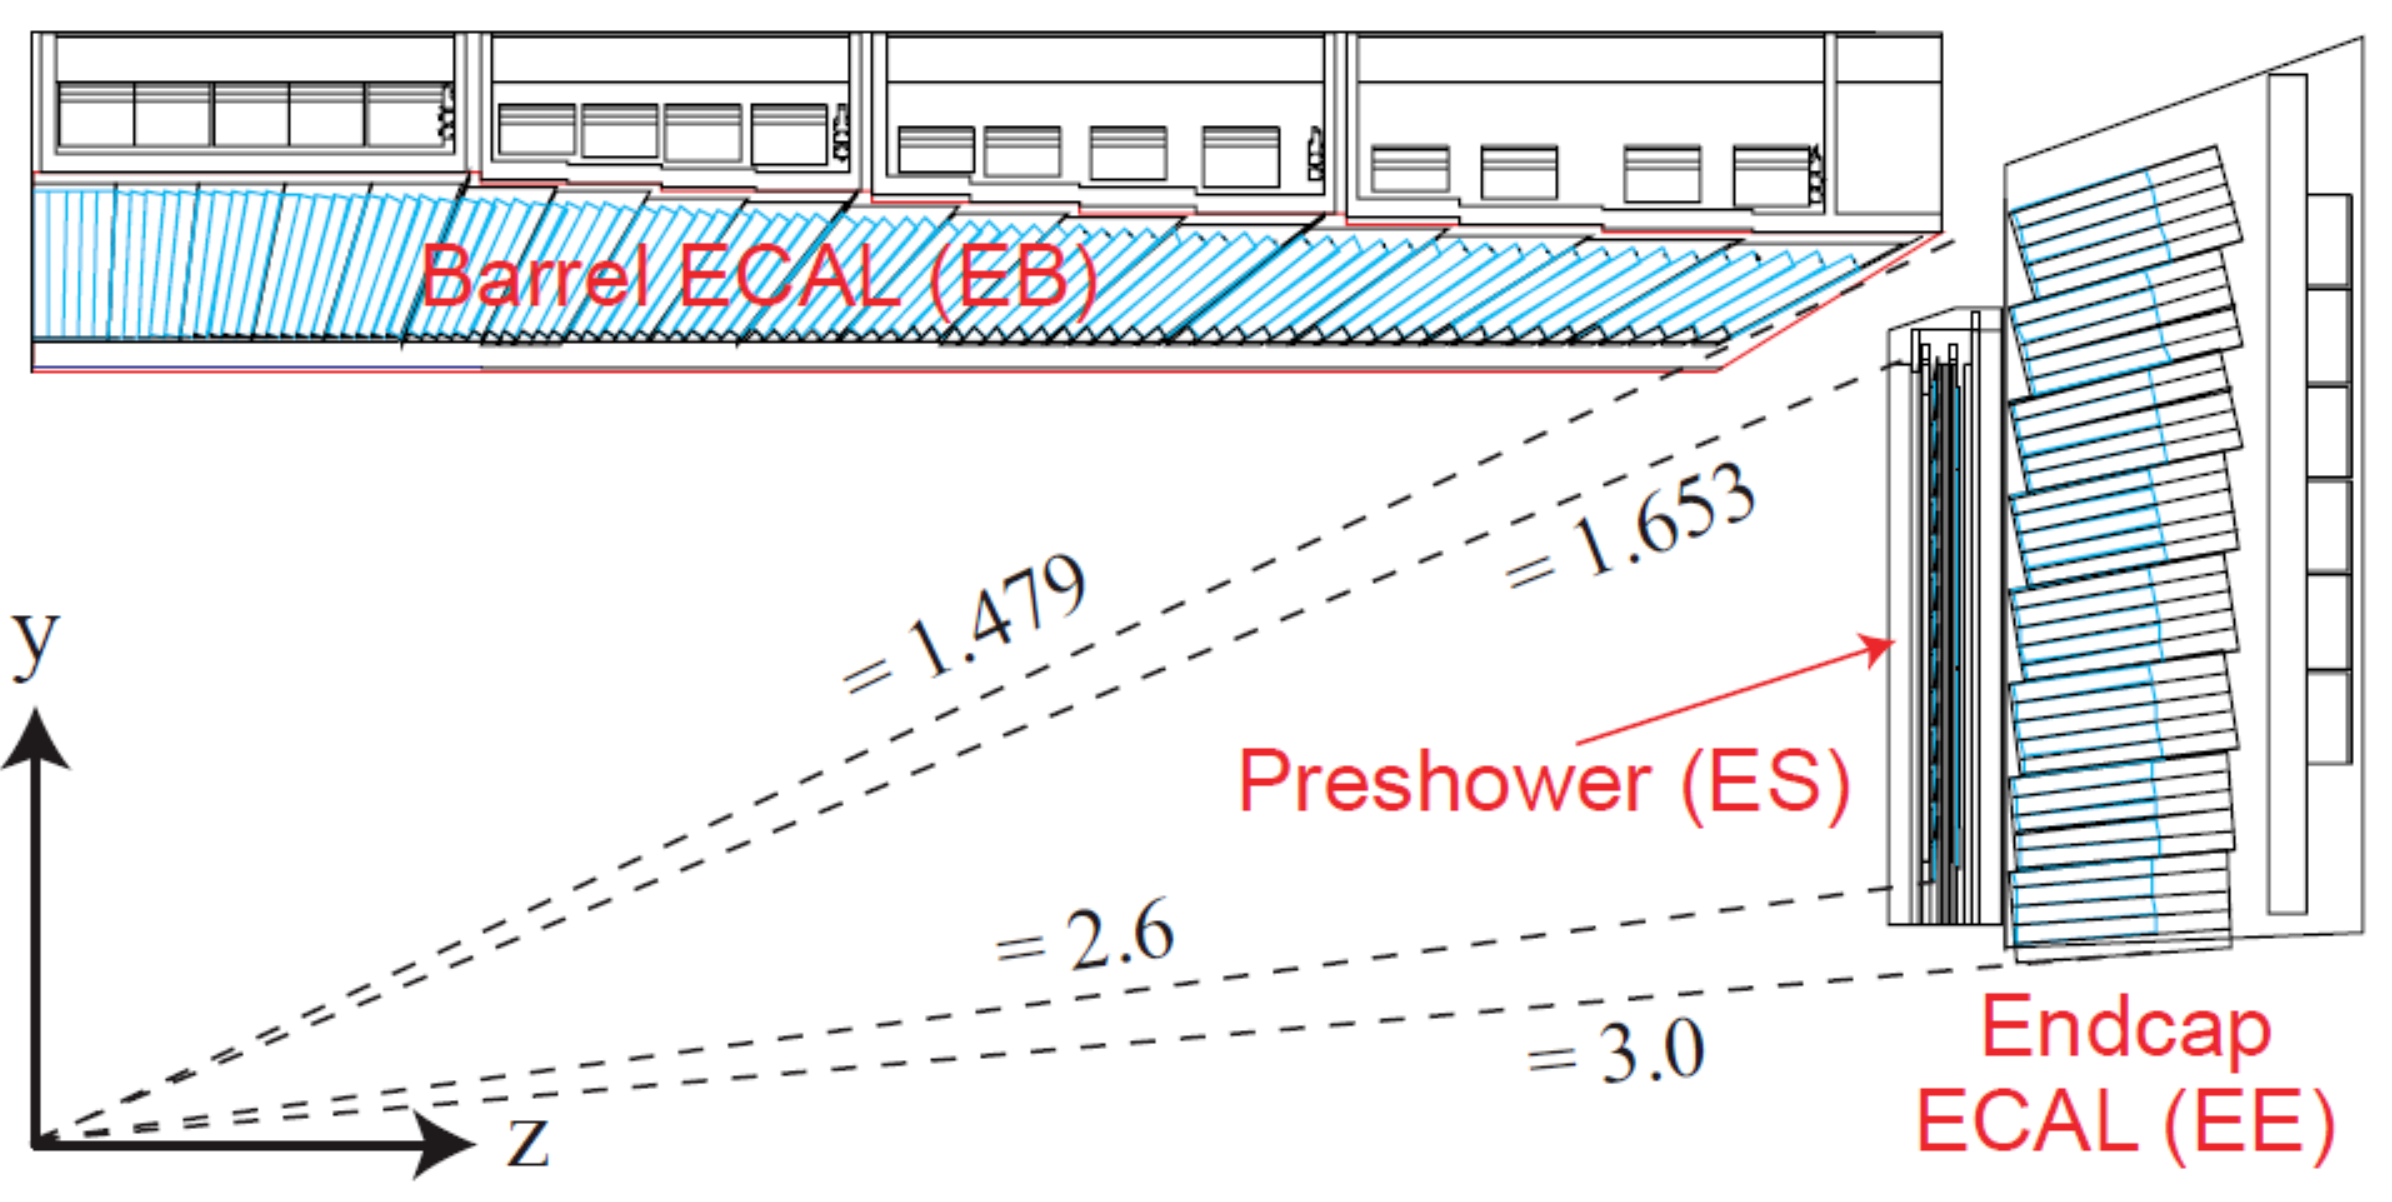
\includegraphics[width=\textwidth]{figs/ecal.png}
\caption{Diagram of the ECAL layout, emphasizing the crystal orientation. A small gap in the $\eta$ coverage is seen.}
\label{fig:ecal}
\end{subfigure}
\caption{The CMS electromagnetic calorimeter.}
\end{figure}

\subsection{Preshower}

The preshower is an additional detector which allows for greater spatial hit resolution of calorimeter clusters in the $1.7<|\eta|<2.6$ region. Placed in front of the crystal calorimeter, it consists of a lead absorber, followed by a plane of silicon-strip sensors, followed by another lead absorber, followed by an orthogonal plane of silicon strip sensors. The silicon sensors are $320\mu m$ thick and measure $6.1\times6.1\textrm{cm}^{2}$ per sensor module. Measurements in the two orthogonal directions of each silicon layer are combined to provide more precise shower shape measurements.

The preshower is designed to properly identify photon pairs resulting from high-$p_{T}$ neutral pion decay (98.8\% branching fraction). When a sufficiently high $p_{T}$ pion decays, the daughter photons become collimated to the extent they can not be separately resolved within the ECAL crystals. Proper identification of neutral pions are important as they are copiously produced in high-energy particle collisions. There is a physics motivation for instrumenting this particular region of the ECAL: at least one of the photons from $H\rightarrow\gamma\gamma$ falls within this region of $\eta$. 

\section{Hadronic Calorimeter}

The hadronic calorimeter is responsible for the reconstruction of undecayed hadrons: pions $\pi^{\pm}$, protons $p$, neutrons n, and kaons $K^{\pm}, K^{0}_{L}$. It is composed of 4 distinct components with some amount of overlap. It is divided into barrel ($|\eta|<1.4$, HB), endcap ($1.3<|\eta|<3$, HE), forward ($3<|\eta|<5.2$, HF), and outer ($|\eta|<1.2$, HO) regions  \cite{hcaltdr}. A diagram of the HCAL geometry is seen in Figure~\ref{fig:hcal}.

In the HE and HB, a particle will interact with the brass absorber inducing a shower of secondary particles. These secondary particles in turn may interact with the brass, and so on creating a hadronic shower within the detector. Interspaced within the absorber are clear plastic scintillator which create flashes of light after de-excitation of the scintillating molecules embedded in the plastic. Wavelength shifting fibers are routed throughout the plastic to absorb the light, which is then piped to hybrid photodiodes. Light incident on the photodiodes liberates electrons via the photoelectric effect which are then accelerated onto the surface of a silicon diode which further amplifies and digitizes the signal. The particle energy is therefore measured by collecting light generated by a hadronic shower as the particle is absorbed in the calorimeter.

Each of these detectors consists of 17 alternating layers of 5cm brass and 1cm plastic. The readout of the optical signals are summed into \textit{towers} of size of roughly 0.09x0.09 in $\eta-\phi$, this results in the $\eta$ segmentation seen in Figure~\ref{fig:hcal}, labeled from 1 to 15 for HB and then 18-29 in HE.  Layers of constant color represent depth segmentation of the summed light within a single tower.  e.g. two energy deposits in the central HE may be formed from a single shower. (Upgrades beginning in 2020 will increase this segmentation, as well as update the signal collection to using silicon photomultipliers  \cite{hcalupgrade}.)

The HO sits \textbf{outside} the magnet in the barrel region $|\eta|<1.2$ and collects additional radiation not absorbed in the material in front of it with an additional layer of scintillator planes.

An addition to HB, HO, and HE, there is a steel calorimeter HF which detects radiation in the very forward region $3<|\eta|<5.2$ on each side of the interaction point. This forward region has a very large radiation flux - the majority of the proton-proton interactions are ``glancing blows'' in which there is very little momentum transfer and the particles are deflected only slightly, directly into this region of the detector - this environment requires a different approach than in the rest of the HCAL. Each detector is comprised of 165cm thick steel interspersed with radiation-hard quartz fibers (parallel to the beamlime) to collect light which is read out by photomultipliers. The tower size in this detector is about 0.175x0.175 in $\eta-\phi$.

\begin{figure}
\centering
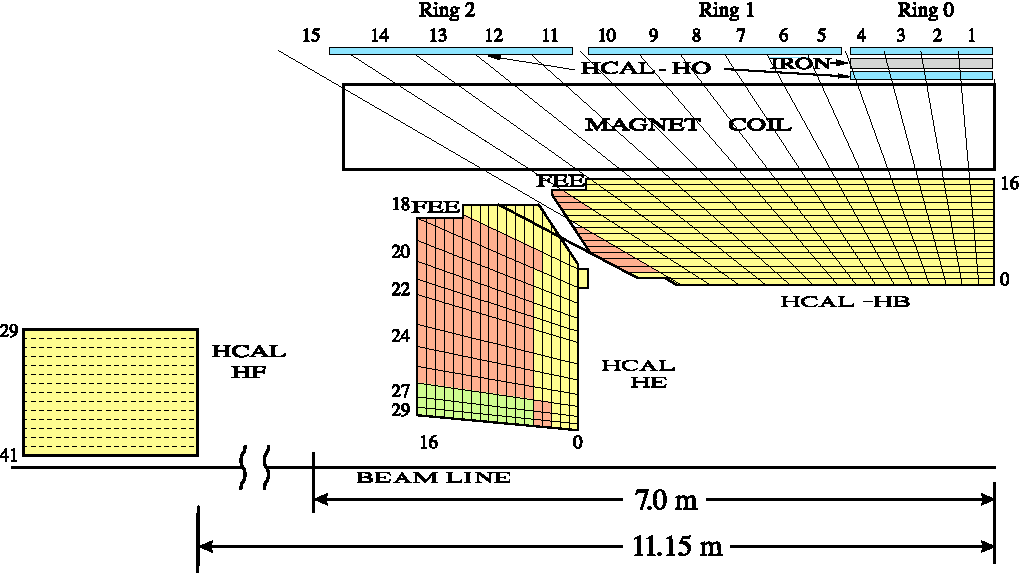
\includegraphics[width=0.8\textwidth]{figs/hcal.pdf}
\caption[The CMS hadron calorimeter.]{The CMS hadron calorimeter \cite{cosmichcal}.}
\label{fig:hcal}
\end{figure}

\section{Solenoidal Magnet}

The solenoidal magnet provides the magnetic field necessary to deflect charged particles within the tracker volume to allow for a measurement of the momentum. The tracker, ECAL, and HCAL all fit inside the magnet bore diameter of 6m and length of 12.5m. It delivers a 3.8T solenoidal field (parallel to the beampipe) within the tracker volume. The field is produced by running current through coils of superconducting NbTi wires cooled to less than 5K. The magnetic field lines are returned via steel yokes sitting outside the magnet interspaced within the muon tracker volume, the field strength throughout the muon system is approximately 2T \cite{magnettdr}. A simulation of the magnetic field within the whole of CMS is seen in Figure~\ref{fig:magnet} \cite{magnet}.

\begin{figure}
\centering
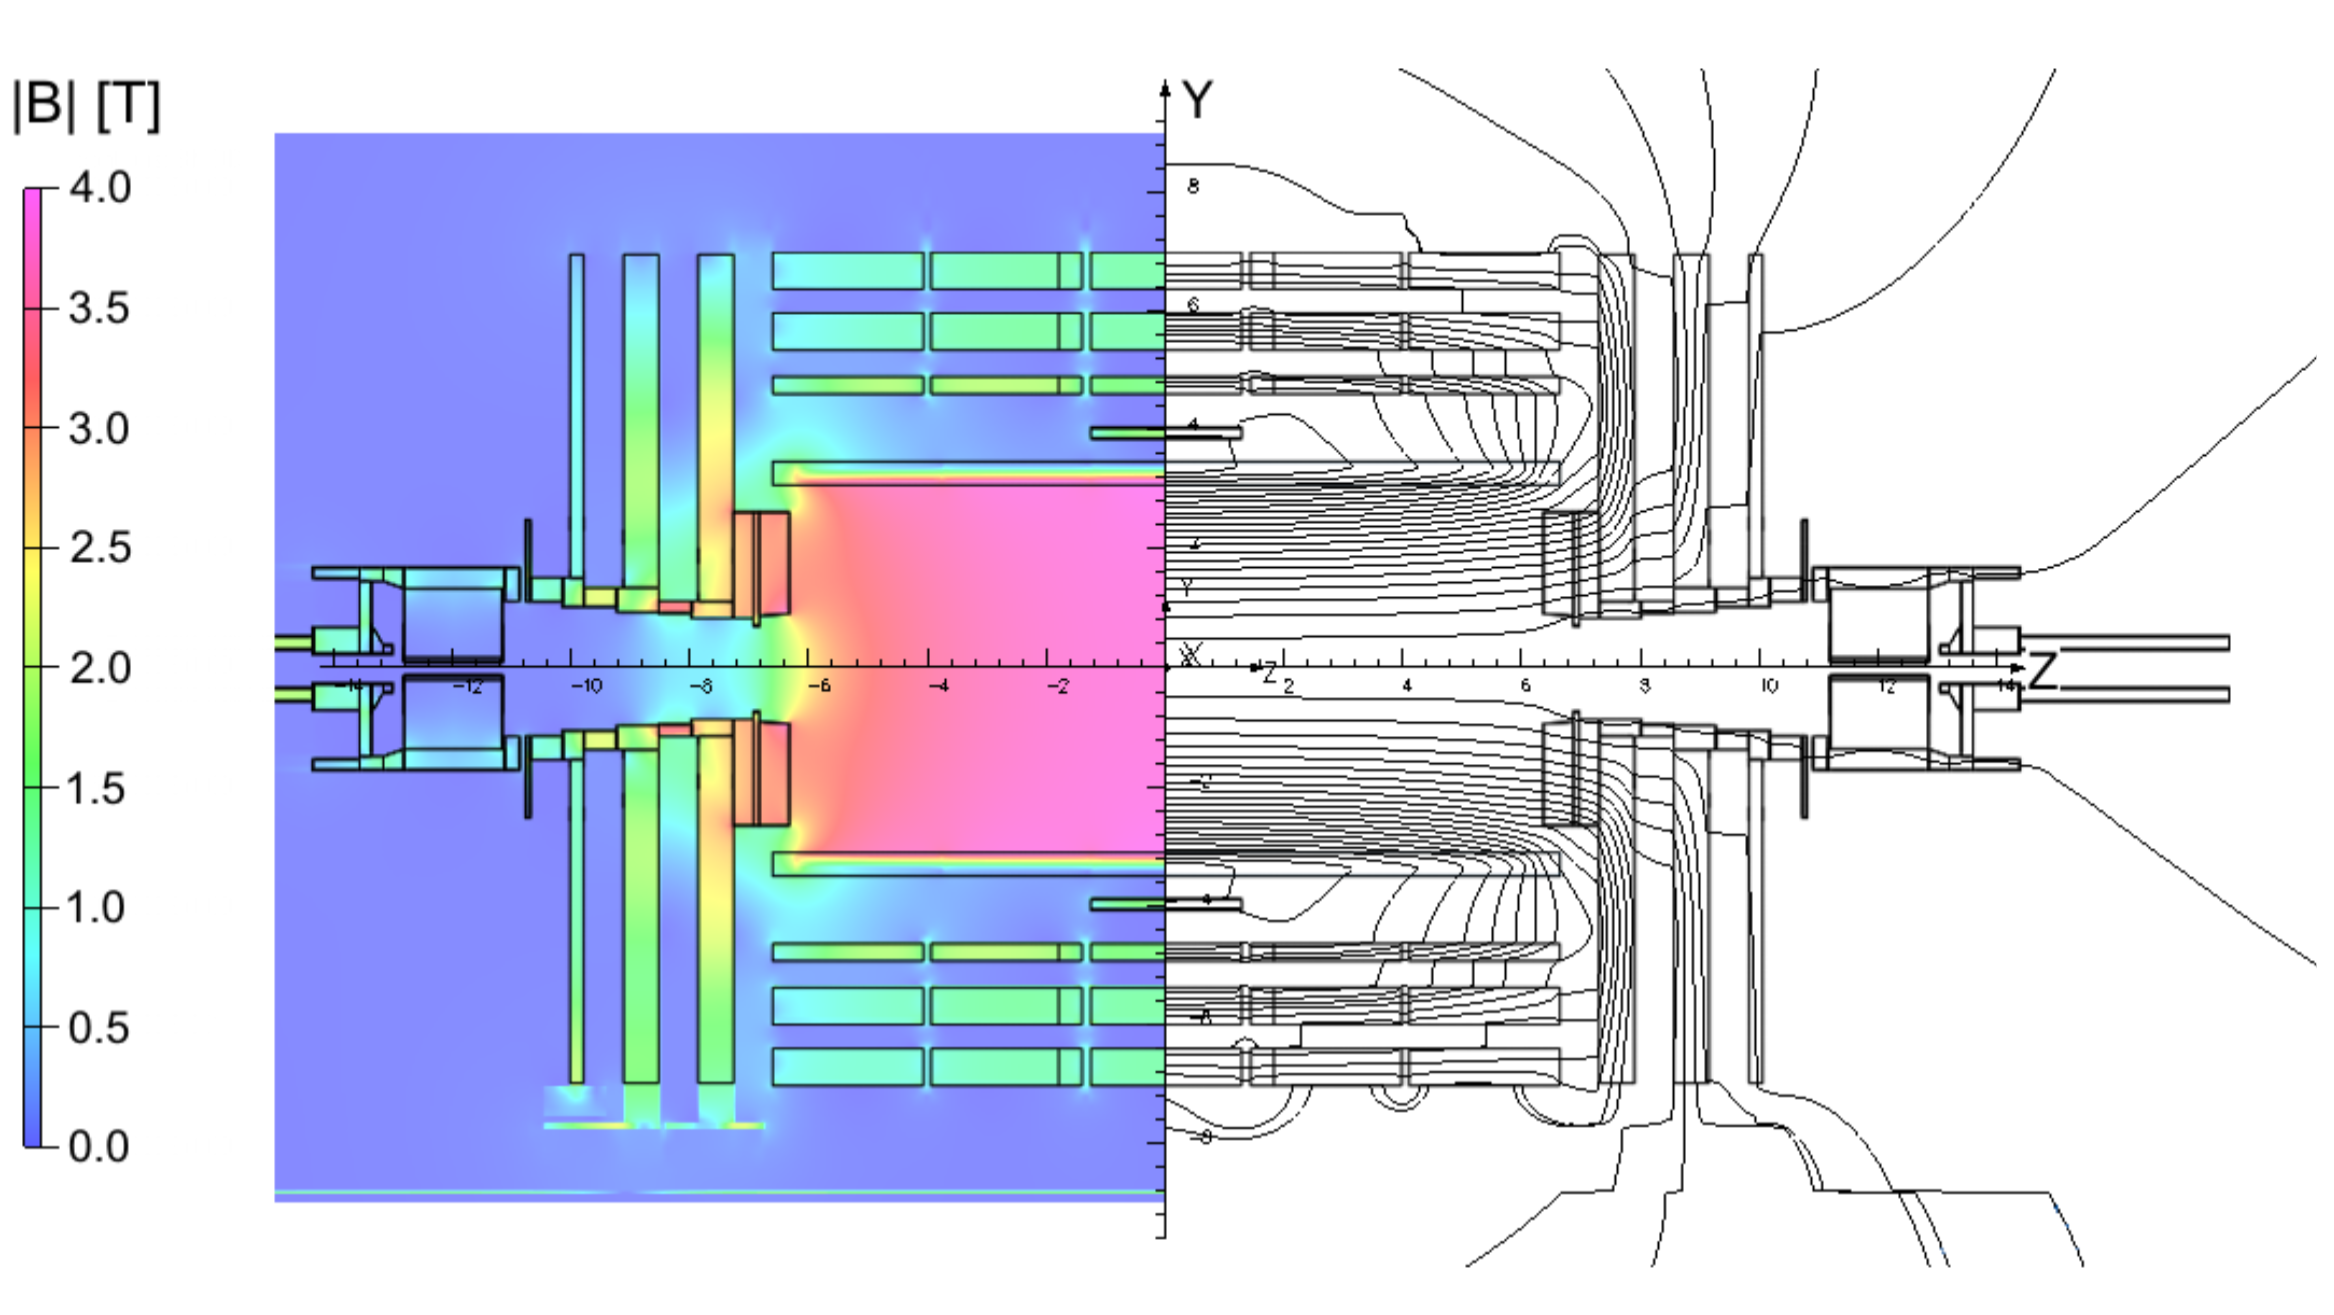
\includegraphics[width=0.7\textwidth]{figs/magnet.png}
\caption[A simulation of the 4T CMS magnetic field.]
{A simulation of the 4T CMS magnetic field. Note the uniformity within the tracker volume.}
\label{fig:magnet}
\end{figure}

\section{Muon System}

The muon system is responsible for the reconstruction (and triggering) of muons $\mu^{\pm}$. The muon trajectory is reconstructed using ionization deposits left in layers of gaseous detectors. The muon momentum is measured by the curvature of the trajectory when immersed in the magnetic field \cite{muontdr}.

The muon system sits at the furthest distance from the beamline, high performance reconstruction is made possible by the balanced combination of the muon and detector properties. Any particles which have made the journey to the muon system has traveled far and through many layers of detector material (e.g. Si, PbWO$_{4}$, Cu), Fe) before finally being detected. Many particles are unstable and decay before reaching the muon system; other particles are absorbed in either of the calorimeters. But the muon has a relatively large mass (compared to an electron) and is not very likely to initiate electromagnetic showers in the ECAL. Nor does the muon interact strongly, and so there will be no hadron showers within the HCAL. Muons have a sufficiently long lifetime to make it to the outer detector. This combination yields a very pure sample of reconstructed muons.

There are three components of the muon system: The drift tubes (DT) are in the barrel ($|\eta|<1.3$), the cathode strip chambers (CSC) are in the endcaps ($0.9<|\eta|<2.4$), and resistive plate chambers (RPC) are in both regions ($|\eta| < 1.6$). These detectors rely on different technology and have some amount of overlap with each other. All detectors participate in triggering and track reconstruction, but the DTs and CSCs provide greater position and momentum resolution, while the RPCs have excellent timing resolution allowing for more precise bunch crossing tagging.

\subsection{Drift Tubes}

The drift tubes are used for muon tracking in the barrel portion of the detector ($|\eta|<1.3$). The basic element is a gas tube 4$\,$x$\,$1.3$\,$cm in transverse size and 2$\,$-$\,$4$\,$m long (depending on its position). High-voltage is applied to a wire strung the length of the cylinder and collects charge released when an incident muon ionizes an 85/15\% Ar/CO$_{2}$ gas mixture \cite{dtperformance}.

The drift tubes are divided into four barrel regions (each called a station) at different radii within the magnetic return yoke. Each station contains 3 \textit{superlayers}, where a superlayer is composed of four layers of stacked tubes, each layer staggered by one half width. For each station, two of the superlayers are oriented parallel to the beamline for $r-\phi$ measurements and one superlayer is perpendicular to the beamline to allow for measurements of the r-z position. An image of a DT station is seen in Figure~\ref{fig:superlayer}.

\begin{figure}
\centering
\begin{subfigure}[c]{0.475\textwidth}
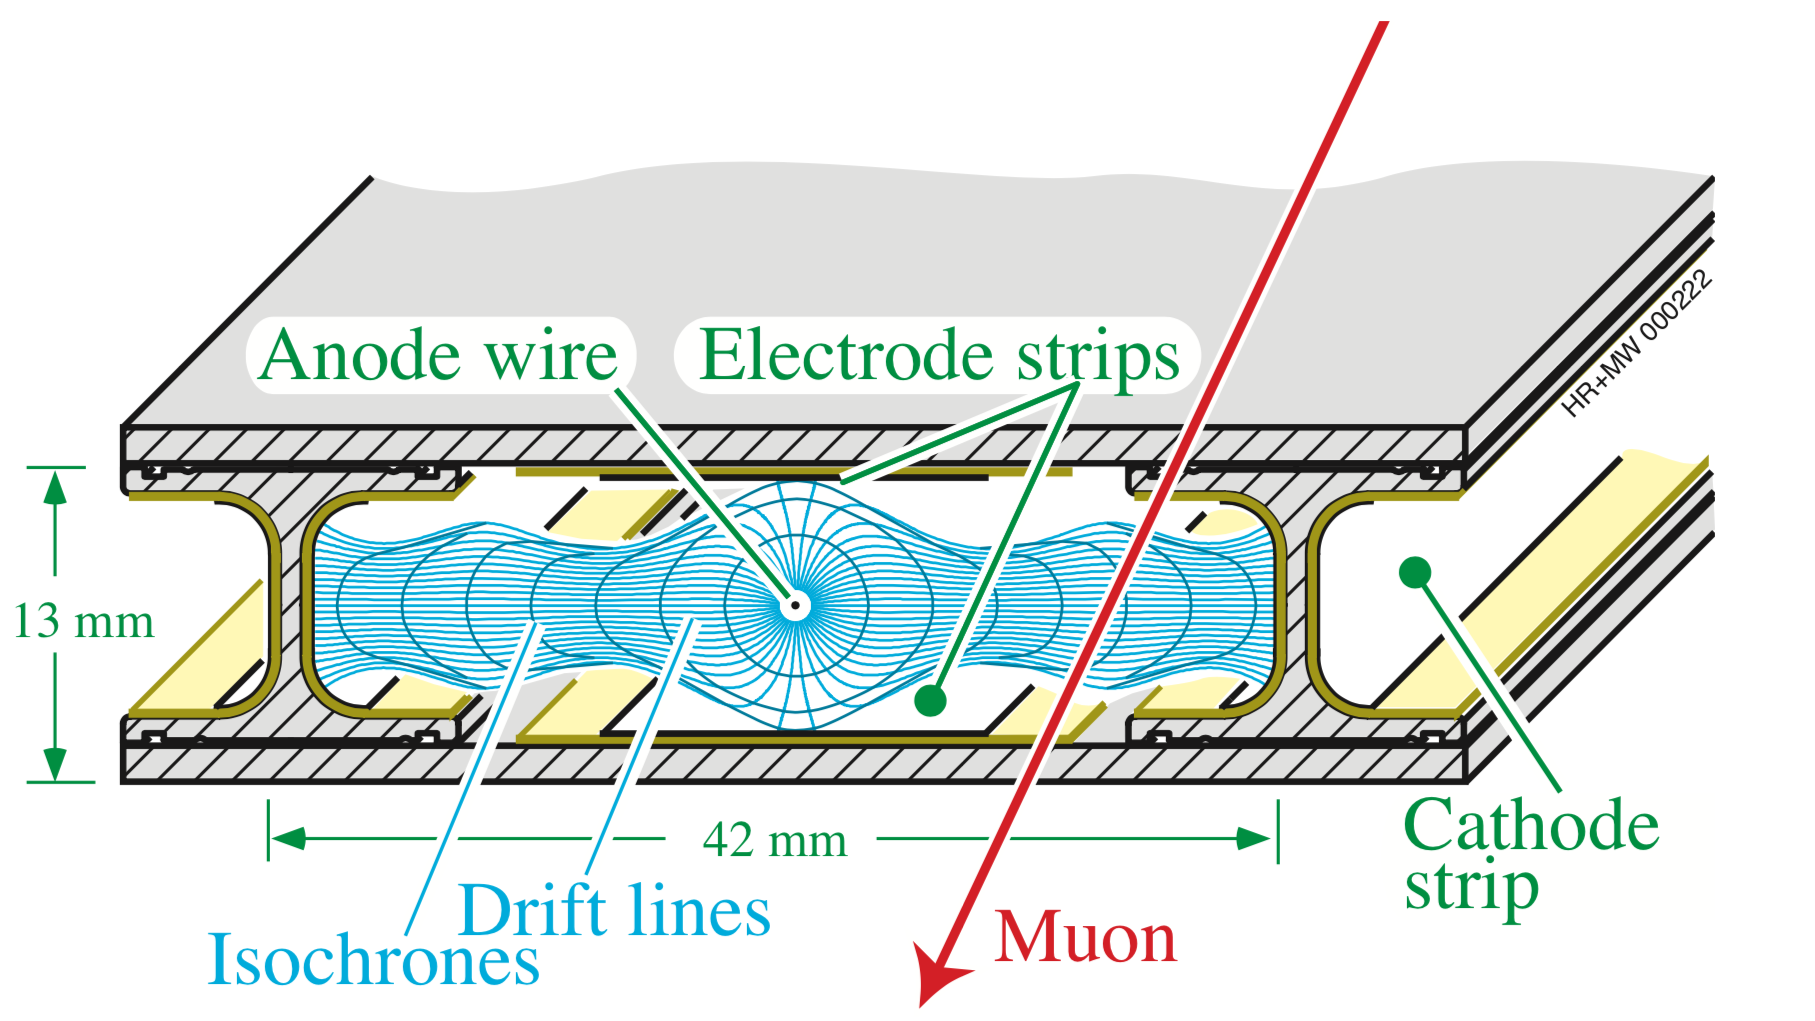
\includegraphics[width=\textwidth]{figs/dtcell.png}
\caption{Cross sectional view of a drift tube cell.}
\end{subfigure}
\begin{subfigure}[c]{0.475\textwidth}
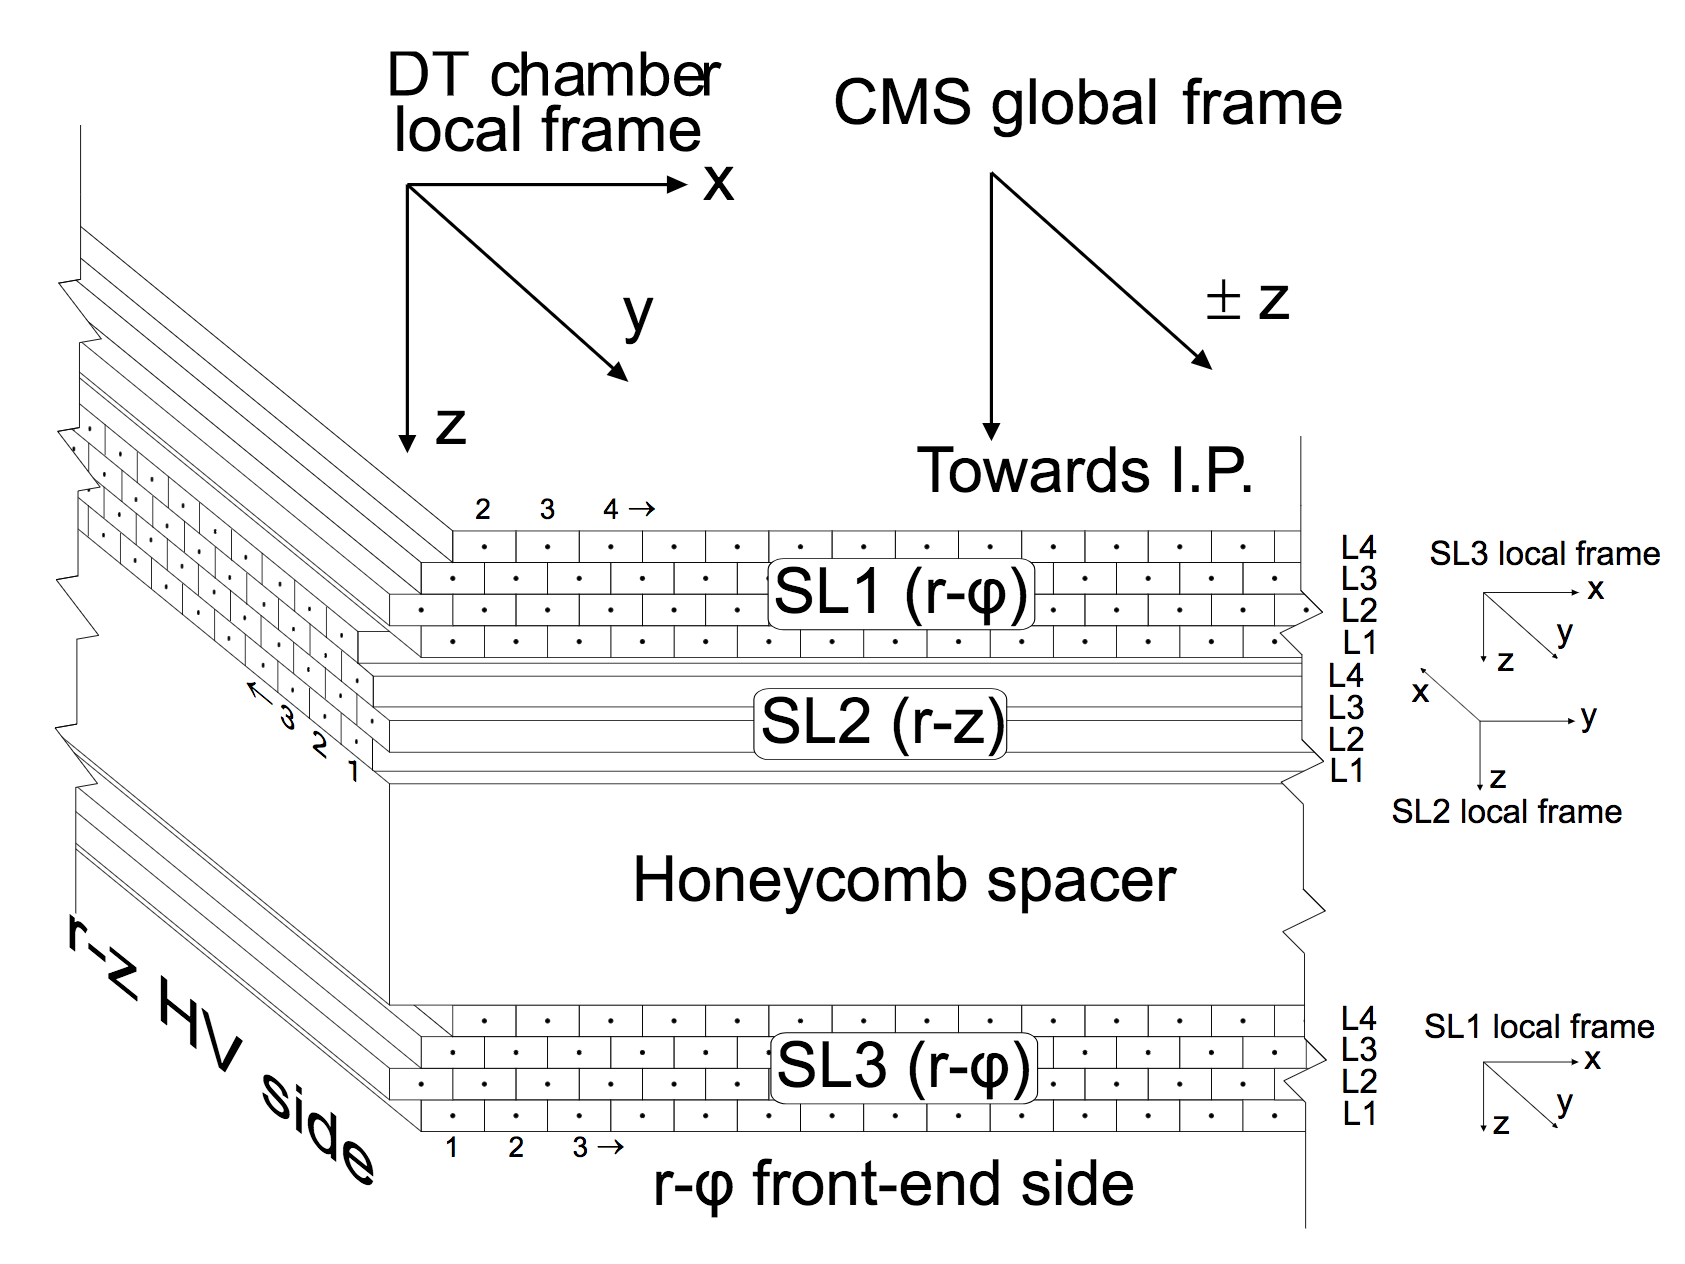
\includegraphics[width=\textwidth]{figs/superlayer.png}
\caption{Drift tube configuration within a superlayer.}
\end{subfigure}
\caption[The CMS muon drift tube detector.]{The CMS muon drift tube detector \cite{dtcellpic}.}
\label{fig:superlayer}
\end{figure}

\subsection{Cathode Strip Chambers}

The cathode strip chambers are used for muon tracking in the endcap portion of the detector ($0.9<|\eta|<2.4$). The system is divided up into 468 trapezoidal chambers arranged in 2 or 3 concentric rings on a disk. There are 4 discs on either side of the detector ($\pm z$). The geometry of the chambers on a disk are seen in Figure~\ref{fig:cscring} (an example image of the hit occupancy of a disc during cosmic ray runs). Each chamber (diagram in Figure~\ref{fig:cscchamber}) consists of 6 layers of electrode planes separated by a gas layer of C$_{2}$H$_{2}$F$_{4}$ (freon) and C$_{4}$H$_{10}$ (isobutane). Wires are strung in the phi direction (concentric circles about the z axis) and therefore make a measurement of the radial coordinate of the hit. The electron shower generates an image charge in cathode planes. For each layer, one of the planes is segmented into strips which are perpendicular to the wires providing an good measure of the $\phi$ coordinate \cite{cscperformance}.

\begin{figure}
\centering
\begin{subfigure}[c]{0.55\textwidth}
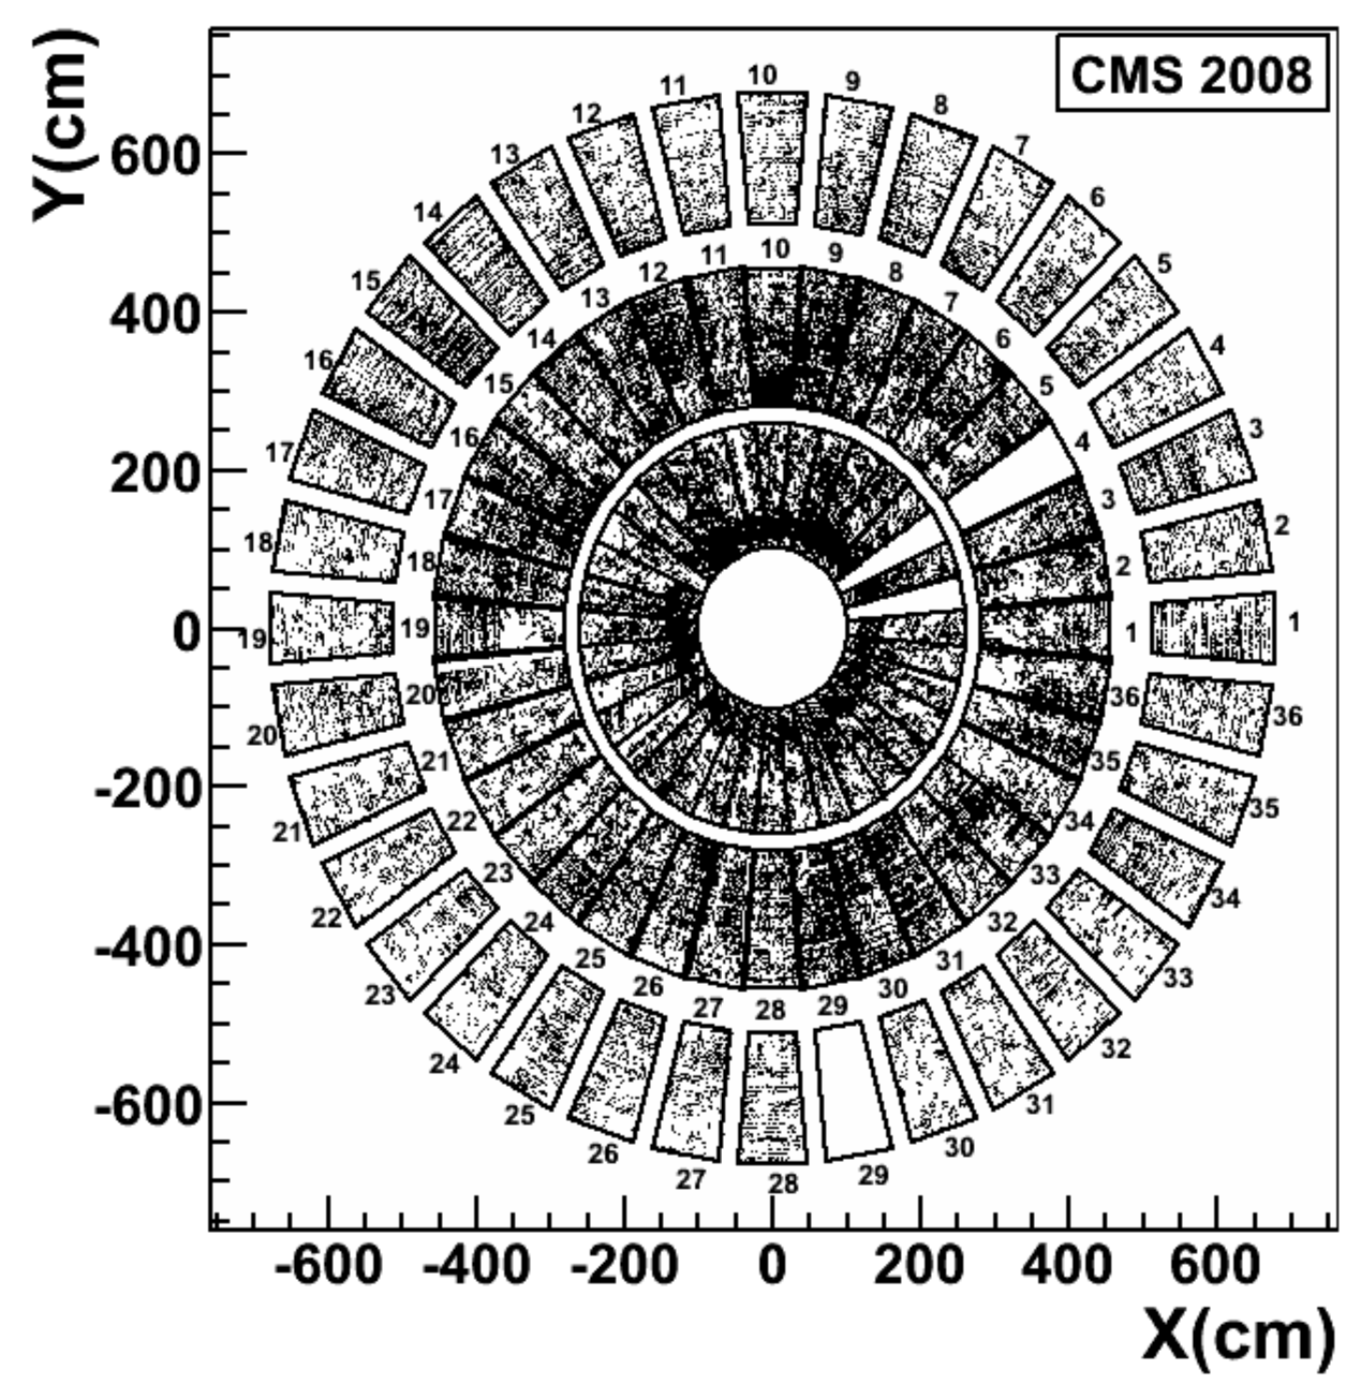
\includegraphics[width=0.8\textwidth]{figs/cscring.png}
\caption[Example occupancy on one CSC disc.]{Example occupancy on one CSC disc \cite{cscperformance}.}
\label{fig:cscring}
\end{subfigure}
\begin{subfigure}[c]{0.3\textwidth}
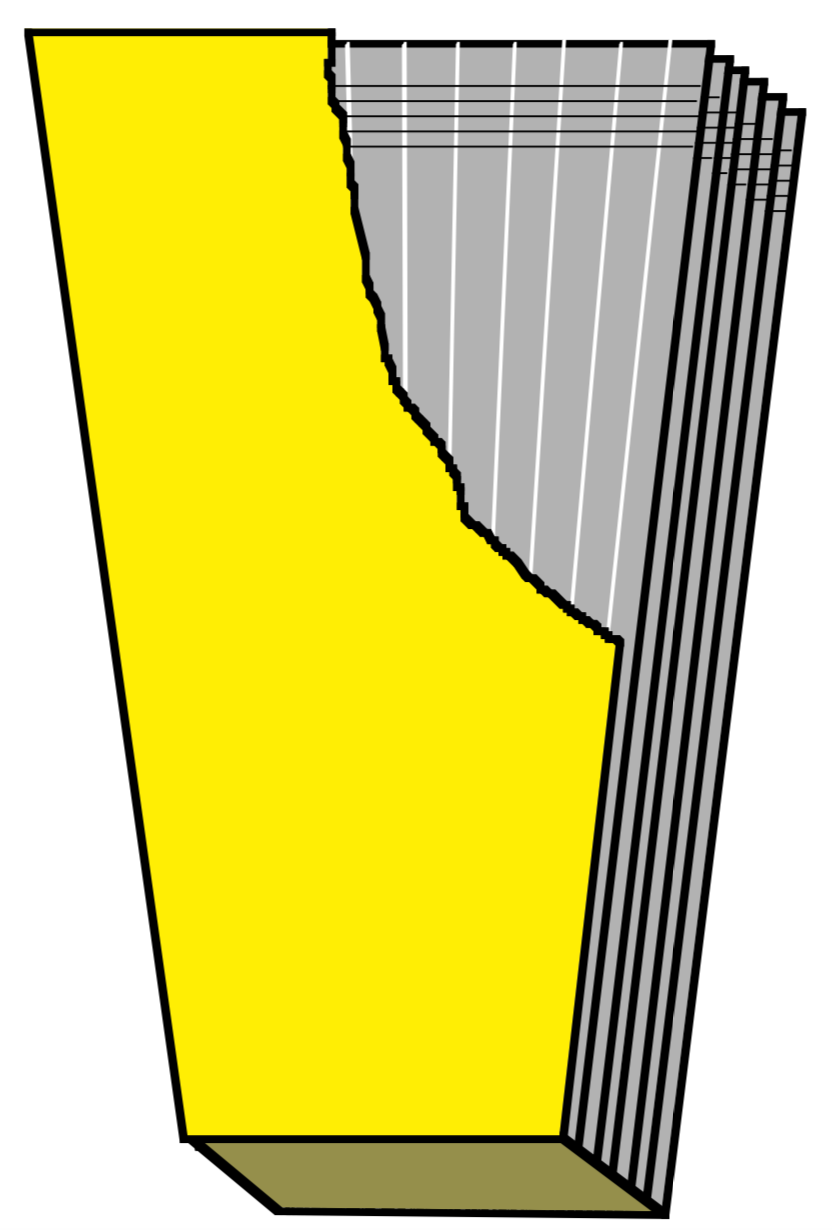
\includegraphics[width=0.9\textwidth]{figs/cscchamber.png}
\caption{One chamber - strips/wires are oriented vertically/horizontally.}
\label{fig:cscchamber}
\end{subfigure}
\caption{The CMS muon cathode strip chambers.}
\end{figure}

\subsection{Resistive Plate Chambers}

Resistive plate chambers cover the region $|\eta| < 1.6$ and are interspersed within CSC and DT and the magnetic return yoke \cite{rpc}. They have an excellent timing resolution of about $3\,\textrm{ns}$ which allows for fast muon triggering and identification of the different bunch crossings. Pattern matching across the hits in the different layers allows for estimates of the muon $p_{T}$ to be used in further trigger processing. Hits created in the resistive plate chambers are additionally used for global fitting of the muon tracks.

The resistive plate chambers consist of an airtight system of two parallel high-resistivity planes separated by a $1\,\textrm{cm}$ gas gap. The outside of each plate is coated to form an electrode for the high-voltage bias. On top of each electrode sits aluminum strips which are insulated from the electrode and serve as the readout. Electron showers created in the gas bulk induce an image charge on the strips which is then recorded. The gas mixture is 95/5\% C$_{2}$H$_{2}$F$_{4}$ (freon) and C$_{4}$H$_{10}$ (isobutane), with trace amounts of SF$_{6}$. A diagram of an RPC chamber is seen in Figure~\ref{fig:rpc}.

\begin{figure}
\centering
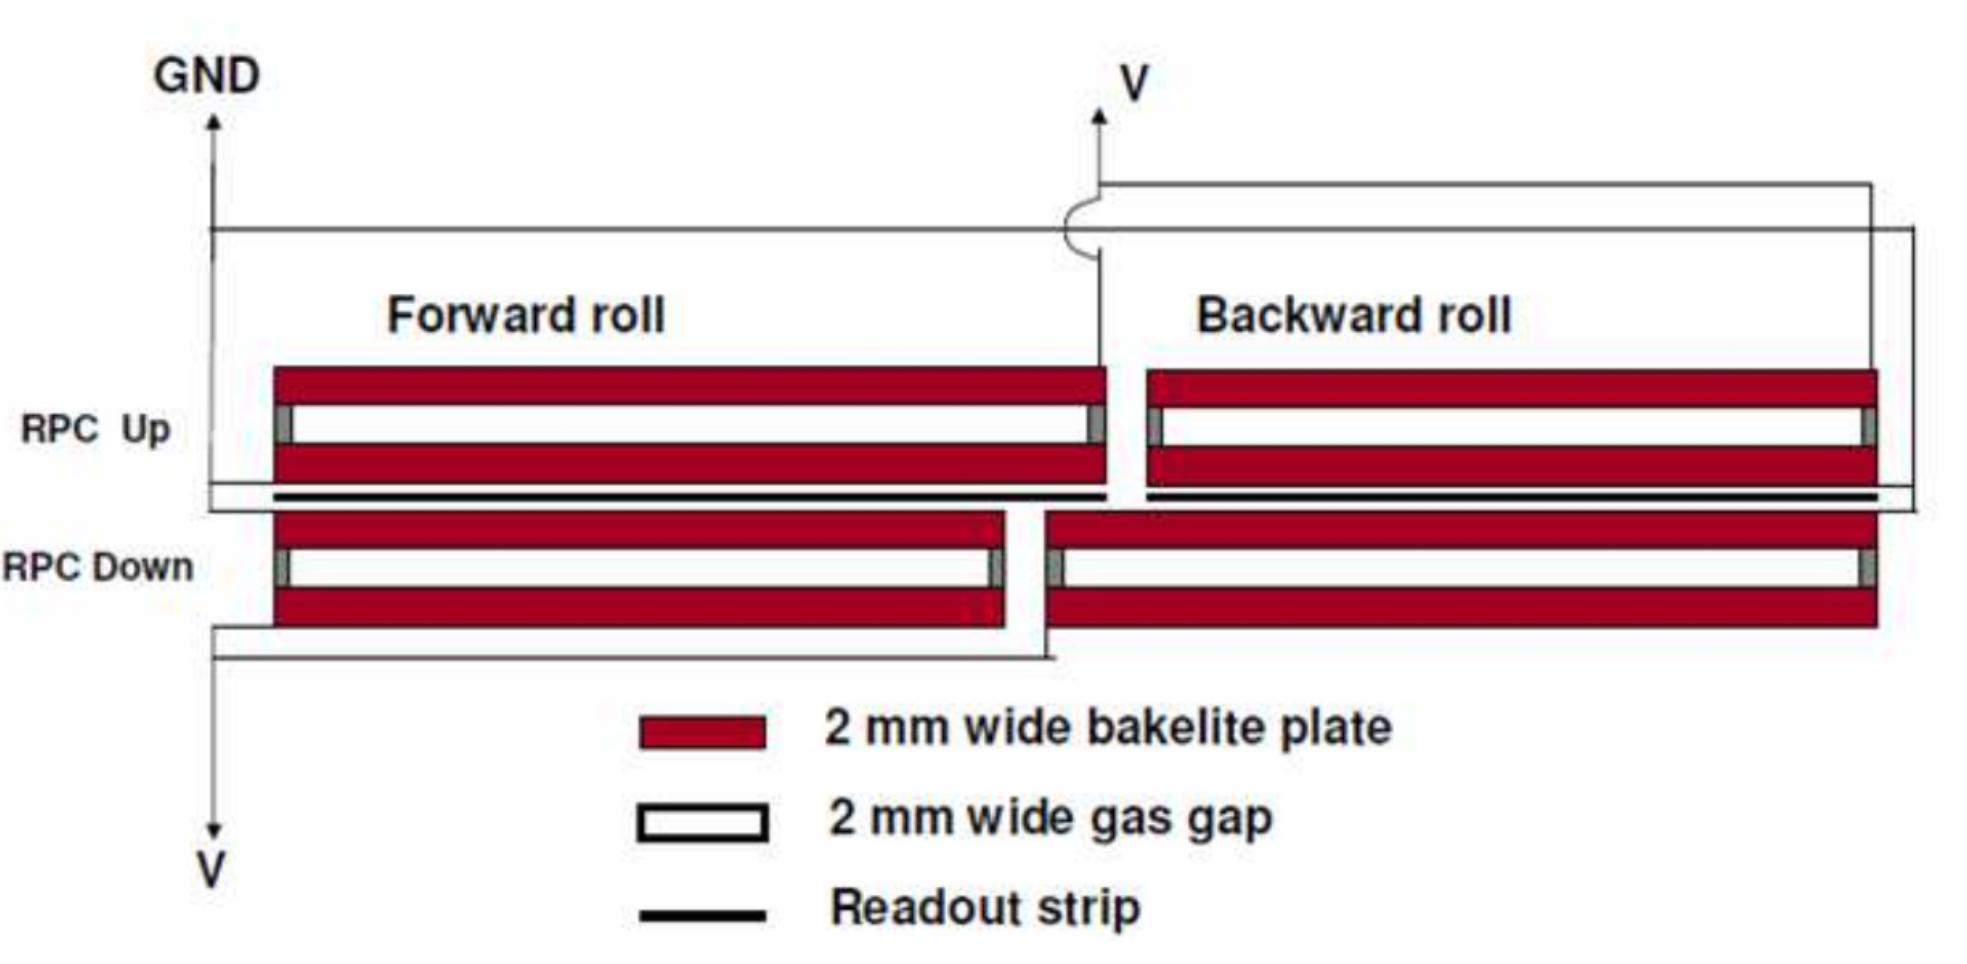
\includegraphics[width=0.6\textwidth]{figs/rpc.png}
\caption[The CMS muon resistive plate chamber.]{The CMS muon resistive plate chamber \cite{rpc}.}
\label{fig:rpc}
\end{figure}

\section{Trigger System}

While in operation mode, the LHC provides collisions at a rate of 40 MHz (25ns per bunchcrossing). This is a phenomenal rate which the CMS detector bandwidth is not able to accommodate, nor does the experiment have access to the amount of storage space necessary to store all this information. Therefore, the CMS detector makes use of a trigger system to quickly determine if the event is 'interesting' and will be saved for storage - events which are not triggered are lost forever. Examples of interesting events are those with high-$p_{T}$ muons, or a large imbalance in the total momentum of the event \cite{CMS-TRG-12-001}.

The trigger consists of two stages known as the Level-1 (L1) and High-Level Trigger (HLT). L1 is a hardware based trigger which combines information from the calorimeters and muon systems to make a decision if the event will be passed to HLT for further processing. L1 is able to reduce the event rate from 40 MHz to 100 kHz and must make the decision within $4\,\mu s$. Primitive objects such as calorimeter energy deposits or muon track segments are first constructed locally within the detector before being combined to form the global decision at L1. If the decision is made at L1 that the event is of potential interest, it is passed to HLT. HLT is a software based trigger which makes use of more sophisticated reconstruction algorithms which can be tuned to select events of choice.

%The flowchart seen in Figure~\ref{fig:trigger} illustrates the L1 system. 
%\begin{figure}
%\centering
%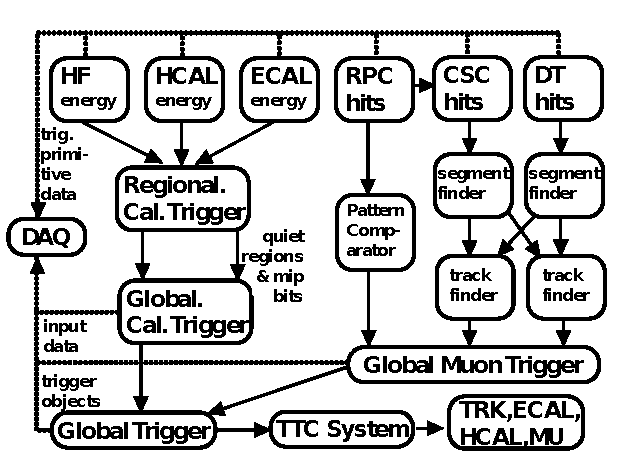
\includegraphics[width=0.6\textwidth]{figs/CMS-TRG-12-001_Figure_002.pdf}
%\caption
%[The CMS L1 trigger system; trigger logic flows from local to global.]
%{The CMS L1 trigger system; trigger logic flows from local (top) to global (bottom).}
%\label{fig:trigger}
%\end{figure}
